\documentclass[tikz]{standalone}
\usepackage{ctex}
\usepackage{tikz}
\usepackage{pgfplots}
\pgfplotsset{compat=1.18}   % 使用较新版本语法
\usetikzlibrary{positioning, arrows.meta, intersections, calc, fit, backgrounds}
\usepgfplotslibrary{fillbetween}  % 用于填充区域
\begin{document}
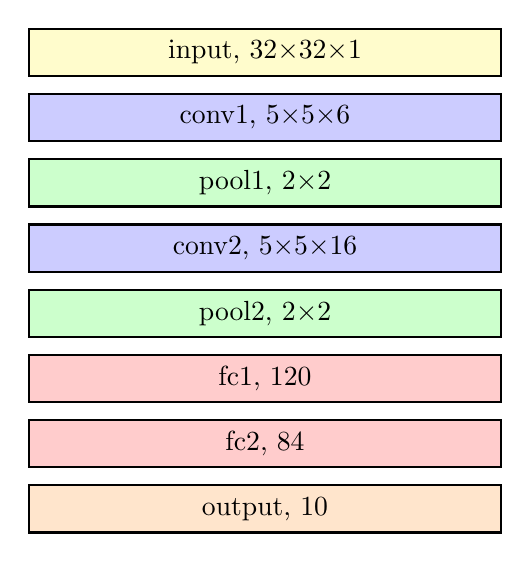
\begin{tikzpicture}[
    ->,>=stealth,shorten >=1pt,auto,thick,
    node distance = 0.2cm,
    >=Stealth,
    conv/.style={draw, minimum width=6cm, minimum height=0.6cm, fill=blue!20},
    pool/.style={draw, minimum width=6cm, minimum height=0.6cm, fill=green!20},
    fc/.style={draw, minimum width=6cm, minimum height=0.6cm, fill=red!20},
    input/.style={draw, minimum width=6cm, minimum height=0.6cm, fill=yellow!20},
    output/.style={draw, minimum width=6cm, minimum height=0.6cm, fill=orange!20},
    activate/.style={draw, minimum width=6cm, minimum height=0.6cm, fill=purple!20},
    norm/.style={draw, minimum width=6cm, minimum height=0.6cm, fill=gray!20},
]
\node[input] (input) {input, 32$\times$32$\times$1};
\node[conv, below=of input] (conv1) {conv1, 5$\times$5$\times$6};
\node[pool, below=of conv1] (pool1) {pool1, 2$\times$2};
\node[conv, below=of pool1] (conv2) {conv2, 5$\times$5$\times$16};
\node[pool, below=of conv2] (pool2) {pool2, 2$\times$2};
\node[fc, below=of pool2] (fc1) {fc1, 120};
\node[fc, below=of fc1] (fc2) {fc2, 84};
\node[output, below=of fc2] (output) {output, 10};

    
\end{tikzpicture}
\end{document}